%!TEX root = ../thesis.tex

\section{実験1 LiDARの反射強度の実験}

\subsection{実験目的}

\newpage

\subsection{壁の反射強度}
  \begin{figure}[h]
    \centering
    \begin{minipage}[c]{65mm} 
        \centering
        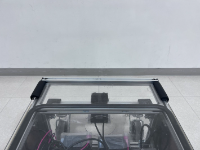
\includegraphics[height=40mm]{images/RobotGuidance_exp1_wall_from_back.png}
        \subcaption{View from behind}
    \end{minipage}
    \begin{minipage}[c]{65mm} 
        \centering
        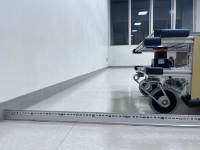
\includegraphics[height=40mm]{images/RobotGuidance_exp1_wall_from_side.png}
        \subcaption{View from the side}
    \end{minipage}
    \caption{Measure the reflection intensity of the wall}
    \label{Fig:RobotGuidance_exp1_wall}
  \end{figure}

\newpage

\subsection{再帰反射テープの反射強度}
  \begin{figure}[h]
    \centering
    \begin{minipage}[c]{65mm} 
        \centering
        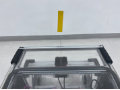
\includegraphics[height=40mm]{images/RobotGuidance_exp2_tape_from_back.png}
        \subcaption{View from behind}
    \end{minipage}
    \begin{minipage}[c]{65mm} 
        \centering
        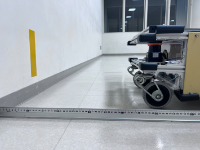
\includegraphics[height=40mm]{images/RobotGuidance_exp2_tape_from_side.png}
        \subcaption{View from the side}
    \end{minipage}
    \caption{Measure the reflection intensity of retroreflective tape}
    \label{Fig:RobotGuidance_exp2_tape}
  \end{figure}

\newpage

\subsection{学習する場所付近の反射強度}
  \begin{figure}[h]
    \centering
    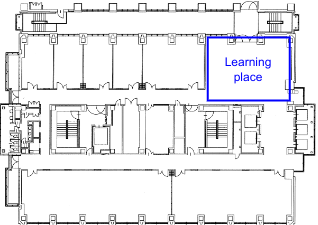
\includegraphics[keepaspectratio, scale=0.80] {images/RobotGuidance_exp3_foyer.png}
    \captionsetup{justification=raggedright} % キャプションを左寄せに
    \caption{Measure the reflection intensity of foyer}
    \label{Fig:RobotGuidance_exp3_foyer}
  \end{figure}

\newpage

\subsection{反射強度を利用した人追従の実験}

\newpage
